\documentclass[10pt]{article}

\usepackage{graphicx}
\usepackage{amsmath,amssymb}
\usepackage{gensymb}
\usepackage{mathtools}
\usepackage{etoolbox}
\usepackage{booktabs}
\usepackage{float}
\usepackage{graphicx}
\usepackage{geometry}
\usepackage{multicol}
\usepackage{caption}

\newcommand\mgin{0.5in}
\geometry{
	left=\mgin,
	right=\mgin,
	bottom=\mgin,
	top=\mgin
}

% Set path to import figures from
\graphicspath{{../figures/}}

% Place converted graphics in current directory
\usepackage[outdir=./]{epstopdf}

% Define multicolumn figure-like environment
% from http://tex.stackexchange.com/questions/12262/multicol-and-figures
\newenvironment{mcfig}
	{\par\medskip\noindent\minipage{\linewidth}}
	{\endminipage\par\medskip}

% Define error function for math mode
\newcommand{\erf}{\mbox{erf}}
% Sign function
\newcommand{\sign}{\mbox{sign}}

% arara: pdflatex
% arara: pdflatex

\begin{document}

%%fakesection Title
\null

\thispagestyle{empty}
\addtocounter{page}{-1}

\begin{center}
    \begin{sffamily}
	\begin{bfseries}
	    \null
	    \vfill
	    \Huge{A Kelp Farming Approach to Sustainable Wastewater Nutrient Removal and Bioenergy Production at Wastewater Treatment Plants with Ocean Outfalls} \\

	    \vspace{20pt}
	    \LARGE{Project Summary} \\
		\LARGE{ASSETs to Serve Humanity NSF REU 2016} \\
	    \vspace{20pt}
    \begin{Large}
		Oliver Evans \\
		Dr. Shane Rogers \\
		Dr. Ole Jacob Broch \\
	\vspace{20pt}
	\today
    \end{Large}
	\end{bfseries}
    \end{sffamily}
    \vspace{30pt}

    \null
    \vfill
    \vfill
    \null
\end{center}
\pagebreak


% Increase table cell height (not for header)
\renewcommand{\arraystretch}{1.5}

\begin{multicols}{2}

\section{Introduction}
The impetus for this project was as follows: Dr. Rogers was approached by the operator of a wastewater treatment plant in Boothbay Harbor, Maine, who is facing increasingly demanding EPA regulations limiting the concentration of certain nutrients that is permissible to release into the ocean via wastewater treatment outfalls.
In order to adhere to these stricter requirements using conventional nutrient remediation, a significant quantity of specialized equipment would be necessary, which is not currently present in the Boothbay Harbor plant.
Being surrounded on all sides by water and private property, the treatment plant has no capacity for the additional necessary equipment, and would therefore need to move their entire operations to a new location in order to conform to these new nutrient regulations.
	As an alternative to conventional processing, Dr. Rogers has proposed the cultivation of the macroalgae \textit{Saccharina Latissima} (sugar kelp) near the outfall site.
The purpose of such an undertaking would be twofold: to sequester the nutrients in question and prevent eutrophication of the surrounding ecosystem, and to reduce one of the primary expenses in macroalgae cultivation: nutrient input.
Once grown, a variety of products can be derived from macroalgae, including biofuel, fish/cattle feedstock, and high value chemical materials such as alginate and agar.
Food for human consumption is also a common product of kelp farming, but it may not be ideal for a wastewater treatment application.
Thus, we seek to investigate the feasibility, potential, and optimal implementation of kelp farming in wastewater treatment operations. 
Specifically, I seek to develop a sophisticated model of the light field in a kelp farming environment as a function of both the spacing and depth of the kelp plants, and of the quality of the water itself.
Ole Jacob Broch is a mathematician at SINTEF, a research organization in Trondheim, Norway, who has been working to model the growth of \textit{Saccharina Latissima} via SINMOD, a large-scale 3D hydrodynamical ocean model developed at SINTEF.
My aim is to develop a light model which can be used both independently and in conjunction with Dr. Broch's SINMOD model.

\section{Physical Setup}
Being a salt water species, macroalgae cultivation occurs primarily in the ocean, with the exception of the initial stage of growth, where microscopic kelp spores are inoculated onto a thread in a small laboratory pool.
This thread is then wrapped around a large rope, which is placed in the ocean and generally suspended by buoys in one of two configurations: horizontal or vertical.
Thus far, I am primarily concerned with modeling the vertical rope case, in which the kelp plants extend radially outward from the rope in all directions.
A \textit{S. Latissima} plant is made up of a single frond (leaf), stipe (stem) and holdfast (root structure).
We consider a rectangular grid of such vertical ropes. 
Each plant will shade both itself and its neighbors to varying degrees based on the depth of the kelp, the rope spacing, the angle of incident light and the nature of scattering in the water.
In addition, light will be naturally absorbed by the water as it travels deeper below the surface, to varying degrees as determined by the clarity of the water.

\section{Overview}
Of primary interest is the radiance at each point from all directions, which affects the photosynthetic rate of the kelp, and therefore the total amount of biomass producible in a given area as well as the total nutrient absorption potential.
The equation governing the radiance throughout the system is known as the Radiative Transfer Equation (RTE), which has been largely unutilized in the fields of oceanography and aquaculture.
Meanwhile, it has been studied extensively in two fields: stellar astrophysics and computer graphics.
In its full form, radiance is a function of 3 spatial dimensions, 2 angular dimensions, and frequency, making for an incredibly difficult problem.
The RTE states that along a given path, radiance is decreased by absorption and scattering out of the path, while it is increased by emission and scattering into the path.
This can be written as
\begin{equation}
	\label{eqn:rte}
	\frac{dR(x,y,z,\theta,\phi)}{d\vec{r}} = -aR -bR + k_e + \int_{4\pi} \beta(\theta,\phi;\theta',\phi') \,d\theta'\,d\phi'
\end{equation}
where $(x,y,z)$ is the point in consideration, $\theta$ and $\phi$ are the azimuth and zenith angles respectively, $\theta'$ and $\phi'$ represent all angles such that $\theta \neq \theta'$ and $\phi \neq \phi'$.

\section{2D Model}
First, let us consider a 2D vertical slab of width $dz$ of a single rope with kelp extending from it.
We assume that the number (not mass) density of kelp plants, $\rho$ is uniform along the length of the rope.

\section{Fundamental assumptions}
We make the following simplifying assumptions to create a framework for the model. Each of these assumptions represents an area of the model which can be further expanded upon to more closely represent the physical system if deemed necessary.
\begin{enumerate}
	\item The frond is two-dimensional. It is flat and does not bend in three dimensions.
	\item The frond has the shape of a kite, as seen in figure \ref{fig:frond}.
	\item The frond is fixed at its base (bottom corner in figure \ref{fig:frond}) to a rope normal to frond, and can rotate freely about that point. The angle which the frond is facing is called $\theta_f$.
	\item The water in which the kelp is situated is flowing at an angle $\theta_w$ with speed $v_w$.
	\item All fronds in the population are geometrically similar.
	\item The population frond length $L$ follows a normal distribution with mean $\mu_L$ and standard deviation $\sigma_L$.
	\item The population frond angle $\theta_f$ follows a von Mises distribution, the circular equivalent of a normal distribution, centered at $v_w$, and whose ``sharpness'' is proportional to $v_w$.
	\item All light arrives from directly above, zenith angle = 0\degree.
	\item All light is absorbed or transmitted, not reflected or scattered.
\end{enumerate}

\section{Frond shape}
\label{sec:shape}

\begin{mcfig}
	\centering
	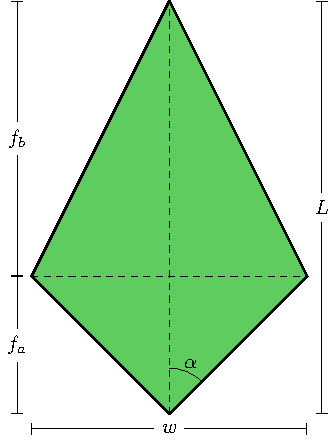
\includegraphics[width=3in]{frond}
	\captionof{figure}{Model frond diagram}
	\label{fig:frond}
\end{mcfig}

The frond is a kite with length $L$ from base to tip, and width $w$ from left to right.
 In figure \ref{fig:frond}, the base is shown at the bottom and the tip is shown at the top.
 The shortest distance from the base to the diagonal connecting the left and right corners is called $f_a$, and the shortest distance from that diagonal to the tip is called $f_b$.
 Clearly,
 \begin{equation}
	 f_a + f_b = L
 \end{equation}
When considering a whole population with varying sizes, it is more convent to specify ratios than absolute lengths.
Let the following ratios be defined.
\begin{align}
	f_r &= \frac{L}{w} \\
	f_s &= \frac{f_a}{f_b}
\end{align}
These ratios are assumed to be consistent among the entire population, making all fronds geometrically similar.
With these definitions, the shape of the frond can be fully specified by $L$, $f_r$, and $f_s$.
It is possible, then, to redefine $w$, $f_a$ and $f_b$ as follows from the preceding formulas.

\begin{align}
	w &= \frac{L}{f_r} \\
	f_a &= \frac{Lf_s}{1+f_s} \\
	f_b &= \frac{L}{1+f_s}
\end{align}

The angle $\alpha$, half of the angle at the base corner, will be important in our analysis.
Using the above equations,
\begin{equation}
	\alpha = \tan^{-1}\left(\frac{2f_rf_s}{1+f_s}\right)
\end{equation}

\section{Variables and functions}
\begin{mcfig}
	\centering
	\begin{tabular}{@{}llc@{}} \toprule
		symbol                    & description                         & model input \\ \midrule
		$L$                       & Frond length                        & \\
		$w$                       & Frond width                         & \\
		$f_a$                     & Inner frond length                  & \\
		$f_b$                     & Outer frond length                  & \\
		$\alpha$                  & Frond shape angle                   & \\
		$\theta_f$                & Frond direction angle               & \\
		$f_s$                     & Frond shape parameter               & \checkmark \\
		$f_r$                     & Frond length-width ratio            & \checkmark \\
		$v_w$                     & Water current speed                 & \checkmark \\
		$\theta_w$                & Water current angle                 & \checkmark \\
		$\mu_L$                   & Pop. mean frond length              & \checkmark \\
		$\sigma_L$                & Pop. frond length std. dev.         & \checkmark \\
		$x,y$                     & Cartesian coordinates               & \\
		$\theta,r$                & Polar coordinates                   & \\
		$\theta_p,r_p$            & Coordinates of point of interest    & \\
		$P_L(L)$                  & Frond length PDF                    & \\
		$C_L(L)$                  & Frond length CDF                    & \\
		$P_{\theta_f}(\theta_f)$  & Frond angle PDF                     & \\
		$P_{2D}(\theta_f,L)$      & 2D length-angle distribution        & \\
		$S(\theta')$              & Angular sign function               & \\
		$r_f(\theta)$             & Frond outer edge function           & \\ 
		$L_{min}(\theta)$         & Min. $L$ value to shade a point     & \\
		$R_s(\theta_p,r_p)$       & Shading region for a point          & \\
		$P_s(\theta_p,r_p)$       & Probability of shading a point      & \\ \bottomrule
	\end{tabular}
	\captionof{figure}{Model quantities. Those marked with a prime (e.g. $x'$) are relative to the frond, as described in section \ref{sec:rel_coords}.}
	\label{fig:variables}
\end{mcfig}

\section{Population distributions}
\label{sec:distributions}
As previously mentioned, the single frond which we are modeling is representative of a population.
While $f_r$ and $f_s$ are held constant among the entire population, $L$ and $\theta_f$ are assumed to vary according to the following distributions.

\subsubsection{Length distribution}
\label{sec:length_dist}
The frond length varies according to a normal distribution with mean $\mu_L$ and standard deviation $\sigma_L$. Since $L>0$, the distribution must be normalized on the positive half-line rather the full line as is standard. The probability density function (PDF) of this distribution is
\begin{equation}
	P_L(L) = e^{-\frac{1}{2}\left(\frac{L-\mu_L}{\sigma_L}\right)^2}
	\cdot \left[ \int_0^\infty e^{-\frac{1}{2}\left(\frac{L-\mu_L}{\sigma_L}\right)^2}\,dL  \right] ^{-1}
\end{equation}

Notice that for a normal distribution,
\begin{equation}
	\displaystyle \lim_{\sigma \to \infty}P(x) = 0 \;\forall x \in \mathbb{R}
\end{equation}

The cumulative density function (CDF) is
\begin{align}
	C_L(L) &= \int_0^L P_L(\xi)\,d\xi  \nonumber \\
	&= \erf\left(\frac{L-\mu_L}{\sqrt{2}\sigma_L}\right)
	\cdot \left[1-\erf \left(\frac{-\mu_L}{\sqrt{2}\sigma_L}\right) \right]^{-1}
\end{align}

where $\erf$ is the error function, defined as 
\begin{equation}
	\erf(x) = \frac{2}{\sqrt{\pi}}\int_0^x e^{-t^2}\,dt
\end{equation}

\begin{mcfig}
	\centering
	\vspace{-1em}
	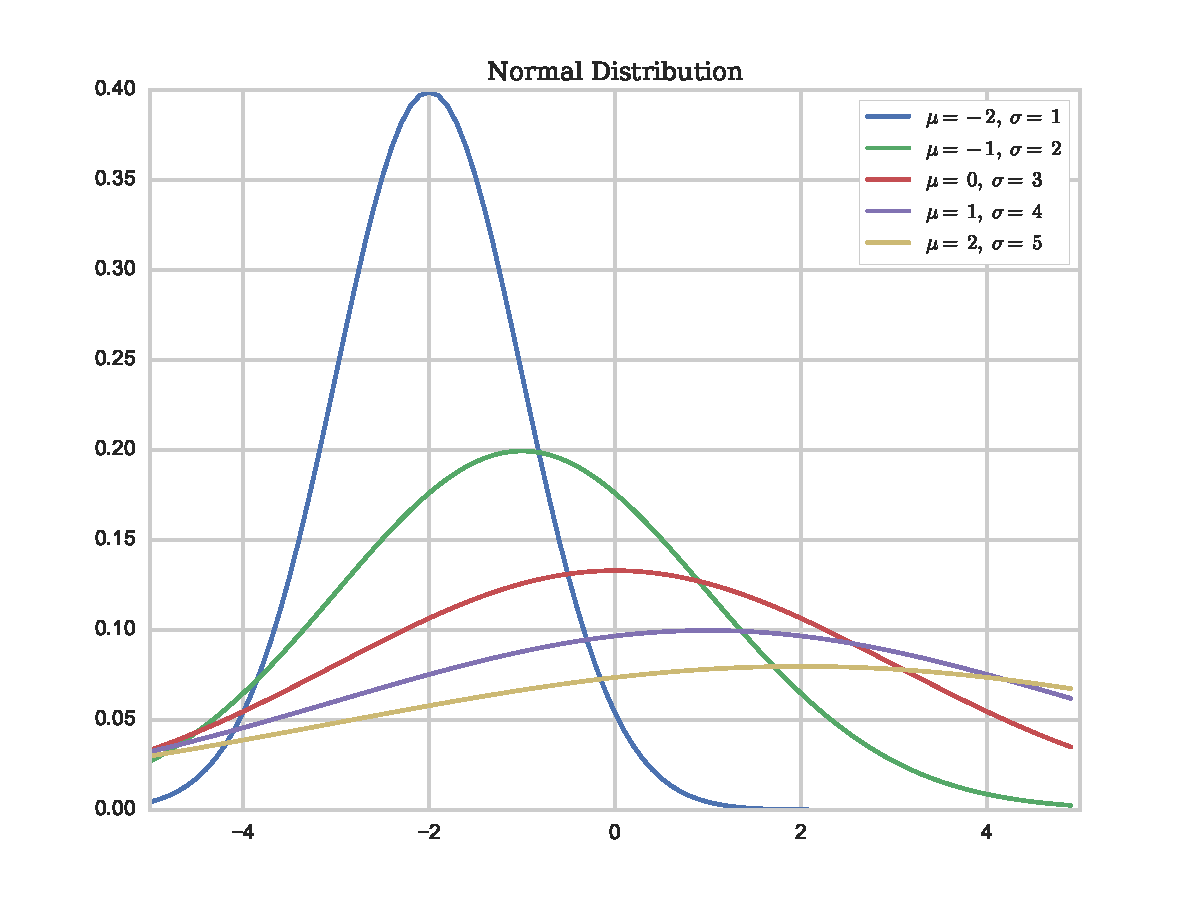
\includegraphics[width=\linewidth]{normal}
	\vspace{-2em}
	\captionof{figure}{Normal distributions for a variety of parameters}
	\label{fig:normal}
\end{mcfig}

\subsection{Frond angle distribution}
\label{sec:angle_dist}
The frond angle varies according to the von Mises distribution, which is the periodic analogue of the normal distribution.
It is defined on $[-\pi,\pi]$ rather than $(-\infty,\infty)$.
It has two parameters, $\mu$ and $\kappa$, which shift and sharpen the distribution respectively.
%$\kappa$ can be considered analogous to $1/\sigma$ in the normal distribution.
Here, we use $\mu = \theta_w$ and $\kappa = v_w$.

The PDF for this distribution is
\begin{equation}
	P_{\theta_f}(\theta_f) = \frac{e^{(v_w)\cos(\theta_f-v_w)}}{2\pi I_0(v_w)}
\end{equation}
where $I_0(x)$ is the modified Bessel function of the first kind of order 0.
Notice that unlike the normal distribution, the von Mises distribution approaches a \textit{non-zero} uniform distribution as $\kappa$ approaches 0.
\begin{equation}
	\displaystyle \lim_{v_w \to 0}P_{\theta_f}(\theta_f) = \frac{1}{2\pi} \;\forall\, \theta_f \in [-\pi,\pi]
\end{equation}
The idea behind using this distribution is that with zero current velocity, the frond angles should be distributed uniformly, while as current velocity increases, they should be increasingly likely to be pointing in the direction of the current.

\begin{mcfig}
	\centering
	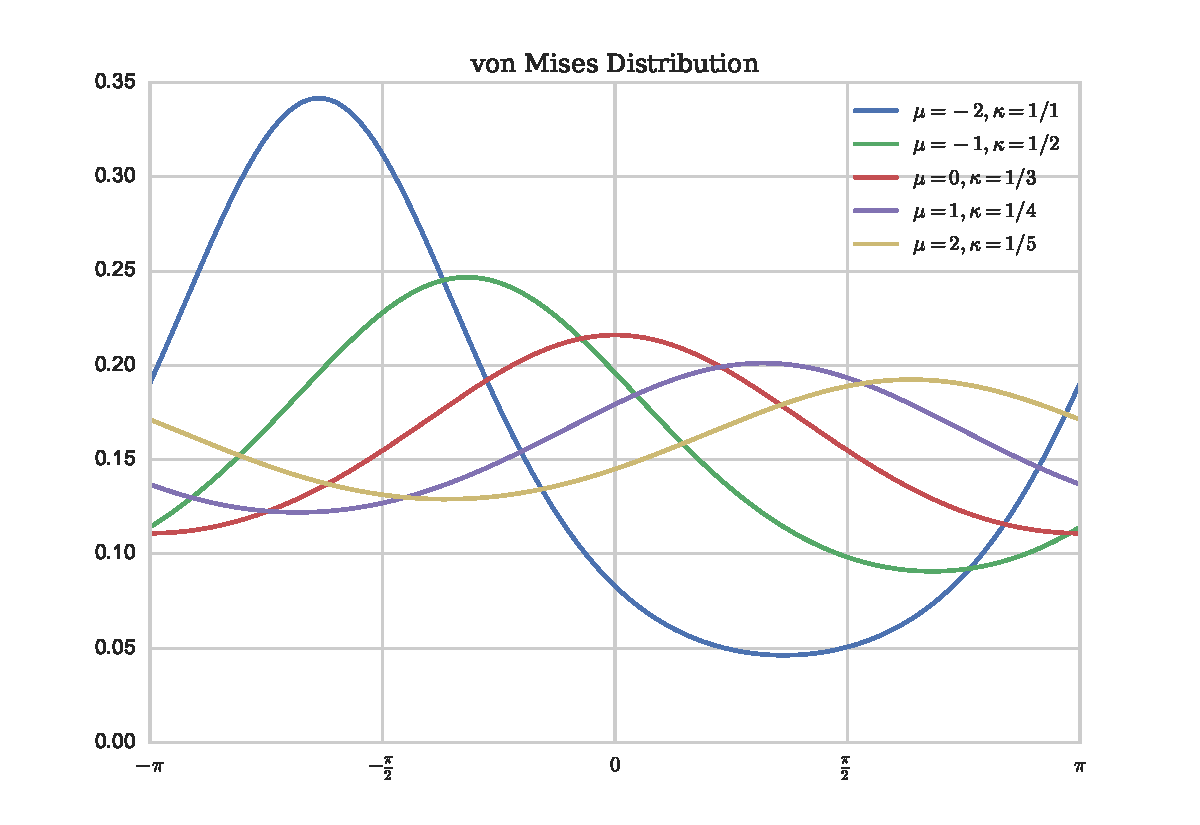
\includegraphics[width=\linewidth]{vonmises_2}
	\captionof{figure}{von Mises distribution for a variety of parameters}
	\label{fig:vonmises}
\end{mcfig}

\subsection{Combined 2D length-angle distribution}
\label{sec:2d_dist}
The previous two distributions are independent of one another. That is, the angle of the frond does not depend on the length, or vice versa.
Therefore, the probability of a frond simultaneously having a given frond length and angle is found as follows.

Given independent events $A$ and $B$,
\begin{equation}
	\label{eq:ind_prob}
	P(A \cap B) = P(A)P(B)
\end{equation}
Then the probability of frond length $L$ and frond angle $\theta_f$ coinciding is 
\begin{equation}
	P_{2D}(\theta_f,L) = P_{\theta_f}(\theta_f) \cdot P_L(L)
\end{equation}
A contour plot of this 2D distribution for a specific set of parameters is shown in figure \ref{fig:dist_2d}, where probability is represented by color in the 2D plane.
Darker green represents higher probability, while lighter beige represents lower probability.
In figure \ref{fig:kelp_sample}, 50 samples are drawn from this distribution and plotted.

It is important to note that if $P_{\theta_f}$ were dependent on $L$, the above definition of $P_{2D}$ would no longer be valid.
For example, it might be more realistic to say that larger fronds are less likely to bend towards the direction of the current.
In this case, equation \ref{eq:ind_prob} would no longer hold, and it would be necessary to use the following more general relation.
\begin{equation}
	P(A \cap B) = P(A)P(B|A) = P(B)P(B|A)
\end{equation}
This is currently not taken into consideration in this model.

\begin{mcfig}
	\centering
	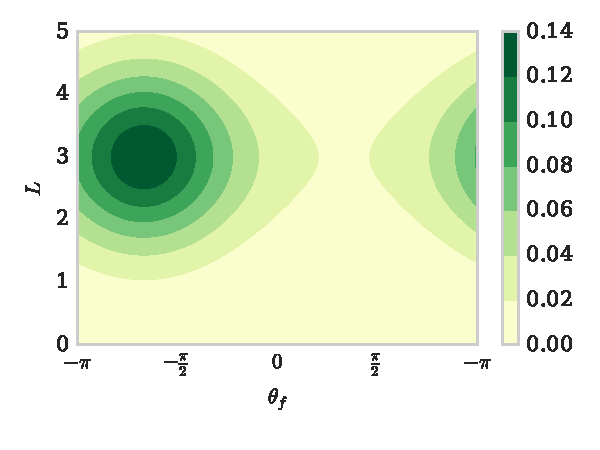
\includegraphics[width=\linewidth]{prob_2d}
	\vspace{-3em}
	\captionof{figure}{2D length-angle probability distribution with \\$\mu_L=3,\sigma_L=1,\theta_f=2\pi/3,v_w=1$}
	\label{fig:dist_2d}
\end{mcfig}

\begin{mcfig}
	\centering
	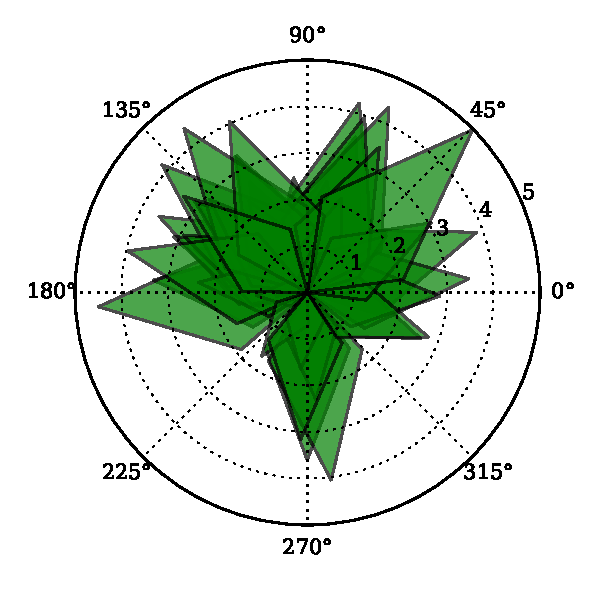
\includegraphics[width=\linewidth]{kelp_sample}
	\vspace{-2em}
	\captionof{figure}{A sample of 50 kelp fronds with length and angle picked from the distribution above with $f_s=0.5$ and $f_r=2$.}
	\label{fig:kelp_sample}
\end{mcfig}

\section{Model Analysis}
\section{Relative coordinate system}
\label{sec:rel_coords}
To determine under what conditions a frond will shade a given point, we begin by describing the shape of the frond in Cartesian and then polar coordinates.
Of primary interest are the edges connected to the frond tip.
For convenience, we will use a relative coordinate system $(\theta',r)$ such that the line connecting the base to the tip is vertical, with the base at $(0,0)$.
The Cartesian analogue of this coordinate system, $(x',y')$, has the following properties.
\begin{align}
	x' &= r\cos\theta' \\ 
	y' &= r\sin\theta'
\end{align}
and
\begin{align}
	r &= \sqrt{x'^2+y'^2}
\end{align}
\vspace{-1em}
\begin{align}
	\theta' &= 
	\begin{cases}
		\tan^{-1}\left( \frac{y}{x} \right) & x > 0 \\
		\tan^{-1}\left( \frac{y}{x} \right) + \pi & x < 0 \\
		\frac{\pi}{2} & x = 0, y > 0 \\
		-\frac{\pi}{2} & x = 0, y < 0 \\
	\end{cases}
\end{align}

\section{Functional description of frond edge}
With this coordinate system established, we can describe the outer two edges of the frond in Cartesian coordinates as a piecewise linear function connecting the left corner: $(-w/2,f_a)$, the tip: $(0,L)$, and the right corner: $(w/2,f_a)$.
This function has the form
\begin{equation}
	y'_f(x') = L-\sign(x')\frac{f_b}{w/2}x'
\end{equation}
where
\begin{align}
	\sign(x) = 
	\begin{cases}
		1 & x > 0 \\
		0 & x = 0 \\
		-1 & x < 0 \\
	\end{cases}
\end{align}

Using the equations in section \ref{sec:rel_coords}, this can be written in polar coordinates after some rearrangement as
\begin{equation}
	r_f'(\theta') = \frac{L}{\sin\theta' + S(\theta')\frac{2f_b}{w}\cos\theta'}
\end{equation}
where
\begin{equation}
	S(\theta') = \sign(\theta'-\pi/2)
\end{equation}

Then, using the relationships in section \ref{sec:shape}, we can rewrite the above equation in terms of our model inputs.
\begin{equation}
	\label{eq:rf_rel}
	r_f'(\theta') = \frac{L}{\sin\theta' + S(\theta')\frac{2f_r}{1+f_s}\cos\theta'}
\end{equation}

\section{Absolute coordinates}
\label{sec:abs_coords}
To generalize to a frond pointed at an angle $\theta_f$, we will use the coordinate system $(\theta,r)$ such that
\begin{equation}
	\theta = \theta' + \theta_f - \frac{\pi}{2}
\end{equation}
Then, for a frond pointed at the arbitrary angle $\theta_f$, the function for the outer edges can be written as 
\begin{equation}
	\label{eq:rf_abs}
	r_f(\theta) = r_f'\left(\theta - \theta_f + \frac{\pi}{2} \right)
\end{equation}

\section{Conditions for shading}
Consider a fixed frond of length $L$ at an angle $\theta_f$. Since light arrives from a zenith angle of 0\degree, a point $(\theta_p,r_p)$ is shaded by the frond if it lies within the region occupied by the frond. That is,
\begin{align}
	\left|\theta_f - \theta_p \right| < \alpha
	\shortintertext{and}
	r_p < r_f(\theta_p)
\end{align}

Equivalently, letting the point $(\theta_p,r_p)$ be fixed, a frond shades the point if the following conditions are satisfied.
\begin{align}
	\theta_p - \alpha < \theta_f < \theta_p + \alpha
	\shortintertext{and}
	L > L_{min}(\theta_p,r_p)
\end{align}
where
\begin{equation}
	L_{min}(\theta) = r_p \cdot \frac{L}{r_f(\theta)}
\end{equation}


Then, considering the point to be fixed, the above equations define the spacial region $R_s(\theta_p,r_p)$ called the ``shading region for $(\theta_p,r_p)$'' with the property that if the tip of a frond lies within this region (i.e. $(\theta_f,L) \in R_s(\theta_p,r_p)$), then it shades the point.
$R_s(3\pi/4,3/2)$ is shown in blue in figure \ref{fig:shade_area} and the smallest possible shading fronds for several values of $\theta_f$ are shown in various colors.
Any frond longer than these at the same angle will also shade the point.

\begin{mcfig}
	\centering
	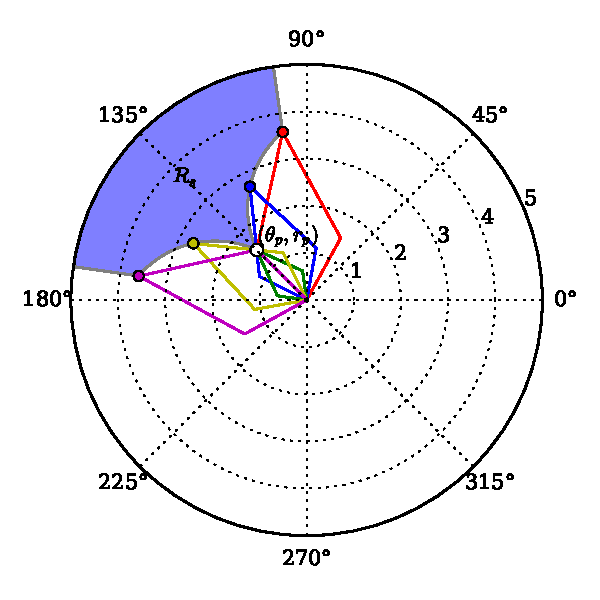
\includegraphics[width=\linewidth]{shade_area}
	\vspace{-2em}
	\captionof{figure}{Outlines of minimum-length fronds for a variety of angles to shade the point $(\theta_p,r_p)=(3\pi/4,3/2)$}
	\label{fig:shade_area}
\end{mcfig}

\section{Probability of shading}
We are interested in the probability that, given a fixed point $(\theta_p,r_p)$, values of $L$ and $\theta_f$ chosen from the distributions described in section \ref{sec:distributions} will fall in the shading region.
This is found by integrating $P_{2D}$ over the shading region for $(\theta_p,r_p)$, as depicted in figure \ref{fig:cart_shade}.

\begin{mcfig}
	\centering
	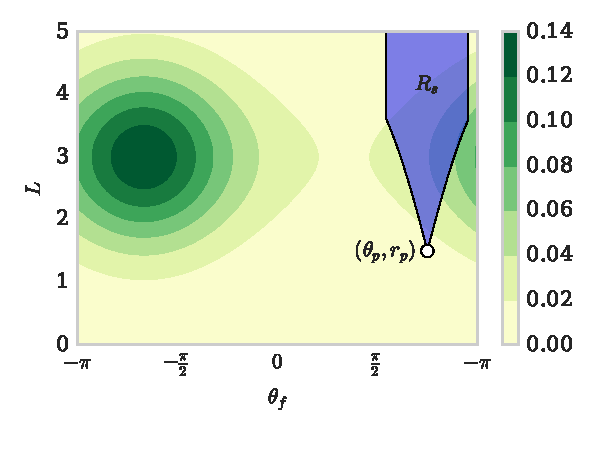
\includegraphics[width=\linewidth]{cart_shade}
	\vspace{-3em}
	\captionof{figure}{Contour plot of $P_{2D}(\theta_f,L)$ overlayed with the region in the $\theta_f-L$ plane which results in shading of the point $(\theta_p,r_p)=(3\pi/4,3/2)$}
	\label{fig:cart_shade}
\end{mcfig}

The probability of a frond shading the point $(\theta_p,r_p)$ is
\begin{align}
		P_s(\theta_p,r_p)	&= \iint_{R_s(\theta_p,r_p)}
								P_{2D}(\theta_f,L)
								\;dL\;d\theta_f \nonumber \\
							&= \int_{\theta_p-\alpha}^{\theta_p+\alpha} 
								\int_{L_{min}(\theta_f)}^\infty
								P_{2D}(\theta_f,L)
								\;dL\;d\theta_f
\end{align}

This integral can be solved numerically as is, or converted to a single integral as follows.
\begin{align}
	P_s(\theta_p,r_p)	&= \int_{\theta_p-\alpha}^{\theta_p+\alpha} 
							\int_{L_{min}(\theta_f)}^\infty
							P_L(L) \cdot P_{\theta_f}(\theta_f)
							\;dL\;d\theta_f \nonumber \\
						&= \int_{\theta_p-\alpha}^{\theta_p+\alpha} 
							P_{\theta_f}(\theta_f)
							\int_{L_{min}(\theta_f)}^\infty
							P_L(L)
							\;dL\;d\theta_f \nonumber \\
						&= \int_{\theta_p-\alpha}^{\theta_p+\alpha} 
							P_{\theta_f}(\theta_f)
							\left[ 1-C_L(L_{min}(\theta_f)) \right]
							\;d\theta_f 
\end{align}

I haven't yet thought of a clever way to evaluate this integral further, so for now, it can be solved numerically in this form.

\begin{mcfig}
	\centering
	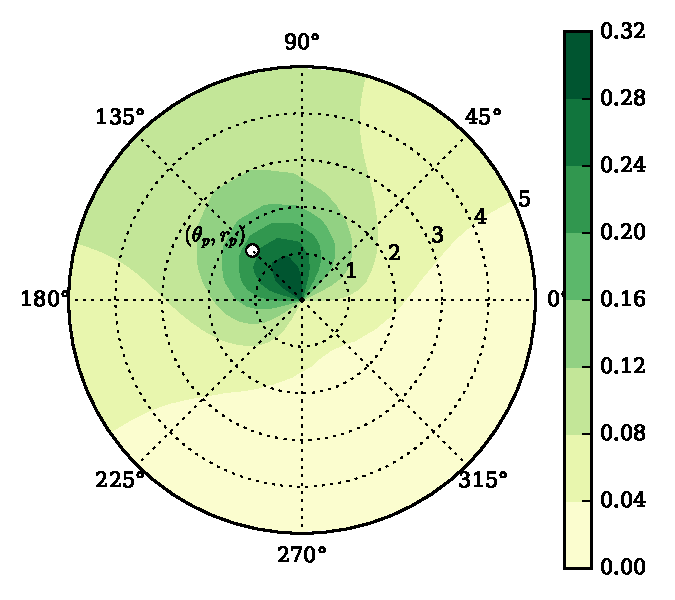
\includegraphics[width=\linewidth]{prob_shade}
	\vspace{-2em}
	\captionof{figure}{Contour plot of the probability of shading sampled at 121 points using $\mu_L=3,\sigma_L=1,\theta_f=2\pi/3,v_w=1$}
	\label{fig:prob_shade}
\end{mcfig}

\section{Big picture, upcoming work}
\section{Model goals}
This work is being done to contribute to the MacroSea project, funded by the Norwegian Research Council, which aims to build a knowledge platform for the industrial cultivation of kelp for use as food, biofuel, and chemical stock among other uses.
Ole Jacob Broch at SINTEF in Trondheim, Norway has been working for several years on developing a system of differential equations to model kelp growth, which is implemented numerically in FORTRAN, and runs in conjunction with SINMOD, a 3D hydrodynamical ocean ecosystem modeling system developed at SINTEF.
My goal is to describe light dynamics in a kelp-farm environment for use in his model.
Ultimately, from this work, we would like to be able to determine the maximum feasible density and depth with which kelp can be cultivated, specifically with regards to light availability and self-shading.

\section{Further development}
Thus far, I have only considered a single frond in two dimensions.
A clear next step will be to extend the model to 3 dimensions, where kelp is radiating from a vertical rope in the water, which is a common cultivation technique.
Fronds could either be treated as discretely spaced or as having a continuous vertical density.
It will then be necessary to also account for attenuation (decay) of light due to other environmental factors, such as water turbidity and phytoplankton concentration.
Ole Jacob's model is discretized into 1m\textsuperscript{3} cubic cells, so perhaps each cube could be treated continuously with frond length and angle distributions as described in section \ref{sec:distributions}, allowing different distributions for different cells.
The light availability and absorption for each cell could be calculated each time step, and the frond distributions for each cell could change as a function of the light absorbed by that cell.

The next step after introducing a third dimension will be to account for multiple ropes each containing many fronds, and considering how fronds on adjacent ropes shade one another.
An important development in this part of the model will be to consider light coming from an angle rather than from directly above.
Potential improvements on the model include accounting for light scattering and reflectance, three dimensional frond rotation, and three dimensional frond bending.
As mentioned in section \ref{sec:2d_dist}, it may also be useful to consider frond length in the angular distribution.
Another interesting idea is to discretize the length and frond angle distributions into a finite number of classes, and use a Markov chain model to describe the movement of fronds between classes, as in the Lefkovitch Matrix method for population dynamics.
This discretization may also improve integration speed to determine the probability of shading.

\section{Alternative methodology}
It may be preferable to consider a finite number of fronds, each with a specific position and angle at each time step, rather than describing fronds probabilistically. This may be difficult considering the increased fluid mechanical complexity and potentially large computational cost of such a simulation.


\end{multicols}
\end{document}


